%
% Diplomarbeit mit LaTeX
% ===========================================================================
% This is part of the book "Diplomarbeit mit LaTeX".
% Copyright (c) 2002-2005 Tobias Erbsland, Andreas Nitsch
% See the file diplomarbeit_mit_latex.tex for copying conditions.
%

\chapter{N�tzliche Pakete}
\index{Pakete}

\section{Anf�hrungszeichen mit dem Paket \enquote{csquotes}}
\index{Anfuehrungszeichen@Anf�hrungszeichen}
\label{sec:anfuehrungszeichen}

Damit Anf�hrungszeichen im gesamten Dokument ein einheitliches Bild abgeben, ist es empfehlenswert das \enquote{csquotes} Paket zu verwenden. Der Vorteil dabei ist, dass durch eine einfache �nderung in der Pr�ambel alle Anf�hrungszeichen im Text ge�ndert werden k�nnen. Wenn du, w�hrend du an der Diplomarbeit schreibst, statt die umgangssprachlich genannten G�nsef��chen neu Guillemets verwenden m�chtest ist das kein grosses Problem. Es reicht dir die Optionen des CSQuote Pakets anzupassen und das Dokument durch den \DMLLaTeX-Kompiler laufen zu lassen.

\subsection{Einbinden des Pakets}

Um das \enquote{csquotes}-Paket zu nutzen bindest du es wie im nachfolgenden Beispiel gezeigt in die die Pr�ambel ein. In den eckigen Klammern wird das Aussehen der Anf�hrungszeichen festgelegt. Gleichzeitig ist es sinnvoll, wenn du dem \enquote{babel}-Paket die Erkennung der Sprache �berl�sst. Ein ganz einfaches Dokument, welches das beschriebene Paket verwendet k�nnte so aussehen:

\lstinputlisting[caption={Einfache Anf�hrungszeichen mit dem \enquote{csquotes} Paket},label=lst:csquotes,frame=tb]{listings/csquotes01.tex}

\begin{description}
\item[Zeile 3] Das Paket \enquote{csquote} wird eingebunden. Mit der Option \texttt{german=quotes} werden die deutschen Anf�hrungszeichen '' bzw ,, verwendet.
\item[Zeile 6] Mit dem Kommando \texttt{\textbackslash enquote\{\}} wird der Text zwischen den Klammern in Anf�hrungszeichen gesetzt.
\end{description}

Durch \verb|german=quotes| werden die Anf�hrungszeichen in Form von '' und ,, gesetzt. Weitere Stile f�r die deutsche Sprache sind Schweizer und franzosische Guillemets ("< und ">). Der Unterschied zwischen den beiden letzteren ist lediglich der Abstand zwischen Anf�hrungszeichen und Text.

\begin{lstlisting}[caption={H�ufig verwendete \enquote{csquotes} Optionen.},label=lst:csquotesoptions,frame=tb]
\usepackage[babel,german=quotes]{csquotes} % Deutsche
\usepackage[babel,german=swiss]{csquotes} % Schweizer
\usepackage[babel,german=guillemets]{csquotes} % Franz�sische
\usepackage[babel,english=american]{csquotes} % Amerikanische
\usepackage[babel,english=british]{csquotes} % Englische
\end{lstlisting}


\subsection{Konfigurieren von TeXnicCenter}

Mit dem Befehl \verb|\enquote{| wird der in Anf�hrunsgzeichen stehende Text begonnen und mit einem \verb|}| abgeschlossen. Durch \verb|\enquote{ }| sind auch Verschachtelungen m�glich. Diese werden durch das Paket automatisch in Ebenen gegliedert und entsprechende der vorgegebenen Optionen gesetzt. Damit du nicht immer \verb|\enquote{| eintippen musst, solltest du in der Konfiguration von TeXnicCenter zwei Ver�nderungen vornehmen. Dadurch wird durch Druck auf die Taste "{} vor einem Wort automatisch \verb|\enquote{| gesetzt, respektiv nach einem Wort die abschliessende geschwungene Klammer.

Klicke im Men� auf \enquote{Extras}, dann auf \enquote{Optionen}. Es �ffnet sich der Optionen-Dialog (Siehe Abbildung \ref{fig:konfiguration05}).

\begin{figure}
	\begin{center}
		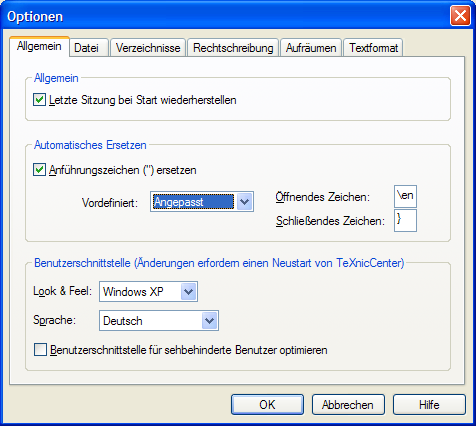
\includegraphics[width=7cm]{images/konfiguration05.png}
		\caption{Konfigurieren der Anf�hrungszeichen}
		\label{fig:konfiguration05}
	\end{center}
\end{figure}

Falls das K�stchen bei \enquote{Anf�hrungszeichen ersetzen} noch nicht markiert ist, markiere es. Danach �nderst du im Pull-Down-Men� den Eintrag auf \enquote{Angepasst} sowie den Eintrag bei \enquote{�ffnendes Anf�hrungszeichen} in \texttt{\textbackslash enquote\{} und bei \enquote{Schlie�endes Anf�hrungszeichen} in \texttt{\}}\footnote{Der Unterschied zwischen den \enquote{Schweizer} und den \foreignquote{french}{Franz�sischen} Anf�hrungszeichen liegt nur im Abstand zwischen Anf�hrungszeichen und Wort. Bei den Schweizer findet sich kein Leerzeichen, bei den Franzosen ein geviert Zwischenraum. Ich verwende in diesem Dokument also die Schweizer, und nicht die Franz�sischen Anf�hrungszeichen.}.

Immer, wenn du jetzt ein einfaches Anf�hrungszeichen (\texttt{''}) eingibst, wird es nun durch ein \textbackslash enquote\{ oder \} ersetzt, je nachdem, ob du dich vor oder hinter einem Wort befindest.

\subsection{Weitere Dokumentation}

Das \enquote{csquotes}-Paket bietet noch eine F�lle an M�glichkeiten, wie zum Beispiel verschiedene Sprachen, Blockquotes und vieles mehr. Die komplette Dokumentation findest du in dem Installationsverzeichniss von MiKTeX unter dem Pfad \enquote{doc\textbackslash latex\textbackslash csquotes}.

